\documentclass[border=0pt]{standalone}
\usepackage{tikz}
\usetikzlibrary{decorations.pathreplacing, calc}

\begin{document}
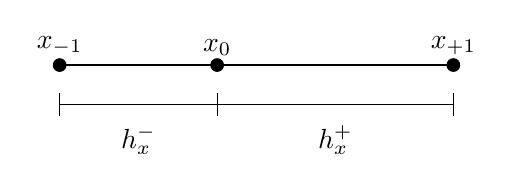
\begin{tikzpicture}[
    % Définir un style pour les lignes de grille verticales
    gridline/.style={draw=black!70, thin}
]

    % Mesh points coordinates

    \coordinate (X-1) at (0, 0);
    \coordinate (X0) at (2, 0);
    \coordinate (X+1) at (5, 0);


    % Points

    %% Draw mesh points and their labels
    \filldraw [black] (X-1) circle (0.08 cm) node[anchor=south]{$x_{-1}$};
    \filldraw [black] (X0) circle (0.08 cm) node[anchor=south]{$x_{0}$};
    \filldraw [black] (X+1) circle (0.08 cm) node[anchor=south]{$x_{+1}$};
    
    %% Connect mesh points with a line
    \draw (X-1) -- (X+1);
    

    % Distances
    
    %% Vertical shift from nodes to distances
    \def\vshift{-0.5cm} 

    %% Draw horizontal distance graduations
    \draw ($(X-1) + (0, \vshift - 0.15cm)$) -- ($(X-1) + (0, \vshift + 0.15cm)$);
    \draw ($(X0) + (0, \vshift - 0.15cm)$) -- ($(X0) + (0, \vshift + 0.15cm)$);
    \draw ($(X+1) + (0, \vshift - 0.15cm)$) -- ($(X+1) + (0, \vshift + 0.15cm)$);
    
    %% Connect with a horizontal line
    \draw ($(X-1) + (0, \vshift)$) -- ($(X+1) + (0, \vshift)$);

    %% Draw distance labels
    \path ($(X-1) + (0, \vshift)$) -- ($(X0) + (0, \vshift)$)
        node[midway, below=0.15cm] {$h_x^-$};
    \path ($(X0) + (0, \vshift)$) -- ($(X+1) + (0, \vshift)$)
        node[midway, below=0.15cm] {$h_x^+$};

\end{tikzpicture}
\end{document}